% % First Chapter : Introduction
%
% Master Thesis: Calibration and Fusion of Stereoscopic and Time-of-Flight 
% Cameras for Zero Gravity Targets Inspection
%
% Achieved at Space System Lab, M.I.T.
% Supervisor: Alvar Saenz-Otero, Daniel Alazard
%
% Institut Sup�rieur de l'A�ronautique et de l'Espace
% Major: Telecommunications et r�seaux - Syst�mes Spatiaux et Lanceurs
% Gabriel Urbain - October 2014
%%

\chapter{Introduction}
\label{chapter:intro}

This document is the result of five-month internship at the Massachusetts Institute of Technology Space System Laboratory (\gls{MIT} SSL) as part of the final project of a double Master degree in Aerospace Engineering, Space Systems and Telecommunications major, at Institut Sup\'erieur de l'A\'eronautique et de l'Espace (\gls{ISAE}), formation SUPAERO and Electrical Engineering, Telecommunications and Multimedia major at Facult\'e Polytechnique of the University of Mons (UMONS). The first chapter introduces the goal and the context of the project to give the reader a global overview of the state-of-art, the \gls{SSL} experience and facilities as well as the new equipment this project focuses on. The second chapter is dedicated to the theoretical aspect and aims at summarizing the required mathematical background and development describing fully and unambiguously every processes. A third chapter analyzes concretely the implementation of the same mechanism from a programmer's point of view. Finally, the results of two different experiment sets will be detailed in the fourth chapter before giving conclusion and future perspectives.

\section{Context}
In many areas of robotics, vision is becoming more and more common in applications such as localization, automatic map construction, autonomous navigation, path following, inspection, monitoring or risky situation detection \cite{visual_navigation}. However, given the features of the cheap sensors currently on the market in the fields of robotics or unmanned vehicles, computer vision is a challenging domain for space navigation. With the increasing performance of embedded computers, the development of faster algorithms and the apparition of new types of devices in the last few years, multi-sensor data fusion is considered as an opportunity to take better advantage of different sensors features to stretch the limits. This project aims at implementing a multi-sensor data fusion algorithm on the space \gls{SPHERES} testbed, as part of the \gls{INSPECT} project. In this perspective, the two stereoscopic cameras of \gls{VERTIGO} and a new Time-of-Flight (\gls{ToF}) camera, also called Optical Range Finder (\gls{ORF}), have been fixed to the Halo hardware of the \gls{SPHERES} nano-satellites. In the future, a thermographic camera will be added to the assembly to increase the data diversity and lead to better results in very dark environments such as spacecrafts in the shadow.

\subsection{\gls{SPHERES}}
\gls{SPHERES} is a facility for demonstrating advanced satellite formation flight, docking, and autonomy algorithms aboard the International Space Station (\gls{ISS}). Created in 1999, \gls{SPHERES} was one of the first educational programs that launched student-designed hardware to the \gls{ISS} in 2006. The ISS contains three SPHERES nano-satellites with fully functional propulsion, guidance, communications, and power systems which enable the nano-satellites to maneuver, communicate with each other and with a laptop control station, and to identify their relative positions.
\begin{figure}[!htt]
	\begin{center}
		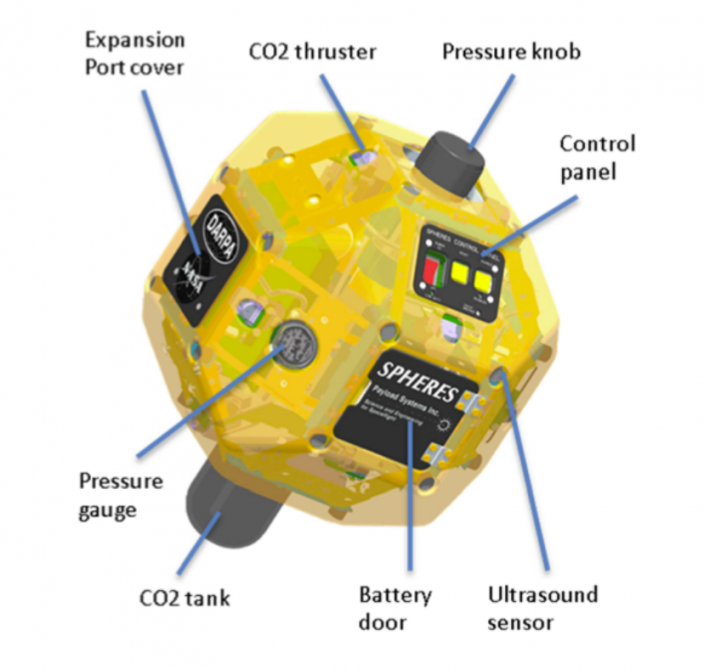
\includegraphics[width=9cm]{img/spheres.png}
		\caption{One of the three \gls{SPHERES} nano-satellites and a brief description of its interfaces.}
		\label{fig:spheres}
	\end{center}
\end{figure}


\subsection{\gls{VERTIGO}}
\gls{VERTIGO} is an extension of the \gls{SPHERES} satellite that develops computer vision navigation and mapping algorithms. Launched in 2012, the \gls{VERTIGO} goggles add to the \gls{SPHERES} satellites a set of stereoscopic cameras and a 1.2 GHz Linux computer that sense the depth of different features on the target object in much the same way as human eyes. Software algorithms running on the compact single-board computer are able to create a detailed three-dimensional map of the unknown, uncooperative and possibly spinning target and estimate its dynamics. The inspector satellite can use this knowledge to plan trajectories around the target achieving autonomous vision-based relative spacecraft navigation.
\begin{figure}[!htt]
\begin{center}
\begin{subfigure}{7.6cm}
  \centering
  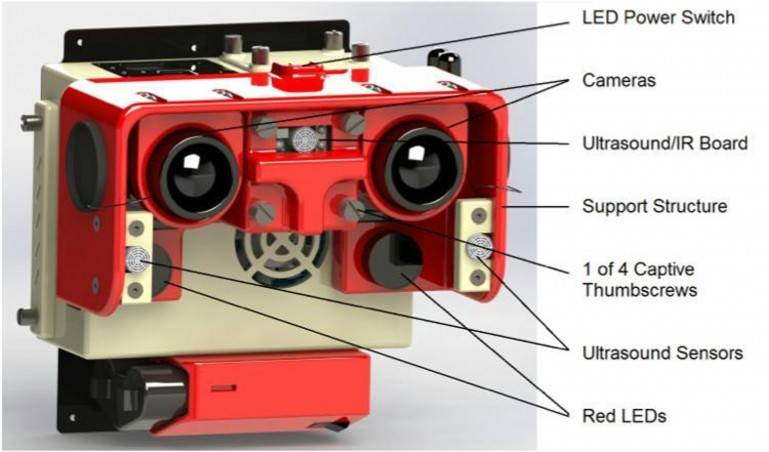
\includegraphics[width=7.5cm]{img/vertigo3.jpg}
\end{subfigure}%
\begin{subfigure}{7.6cm}
  \centering
  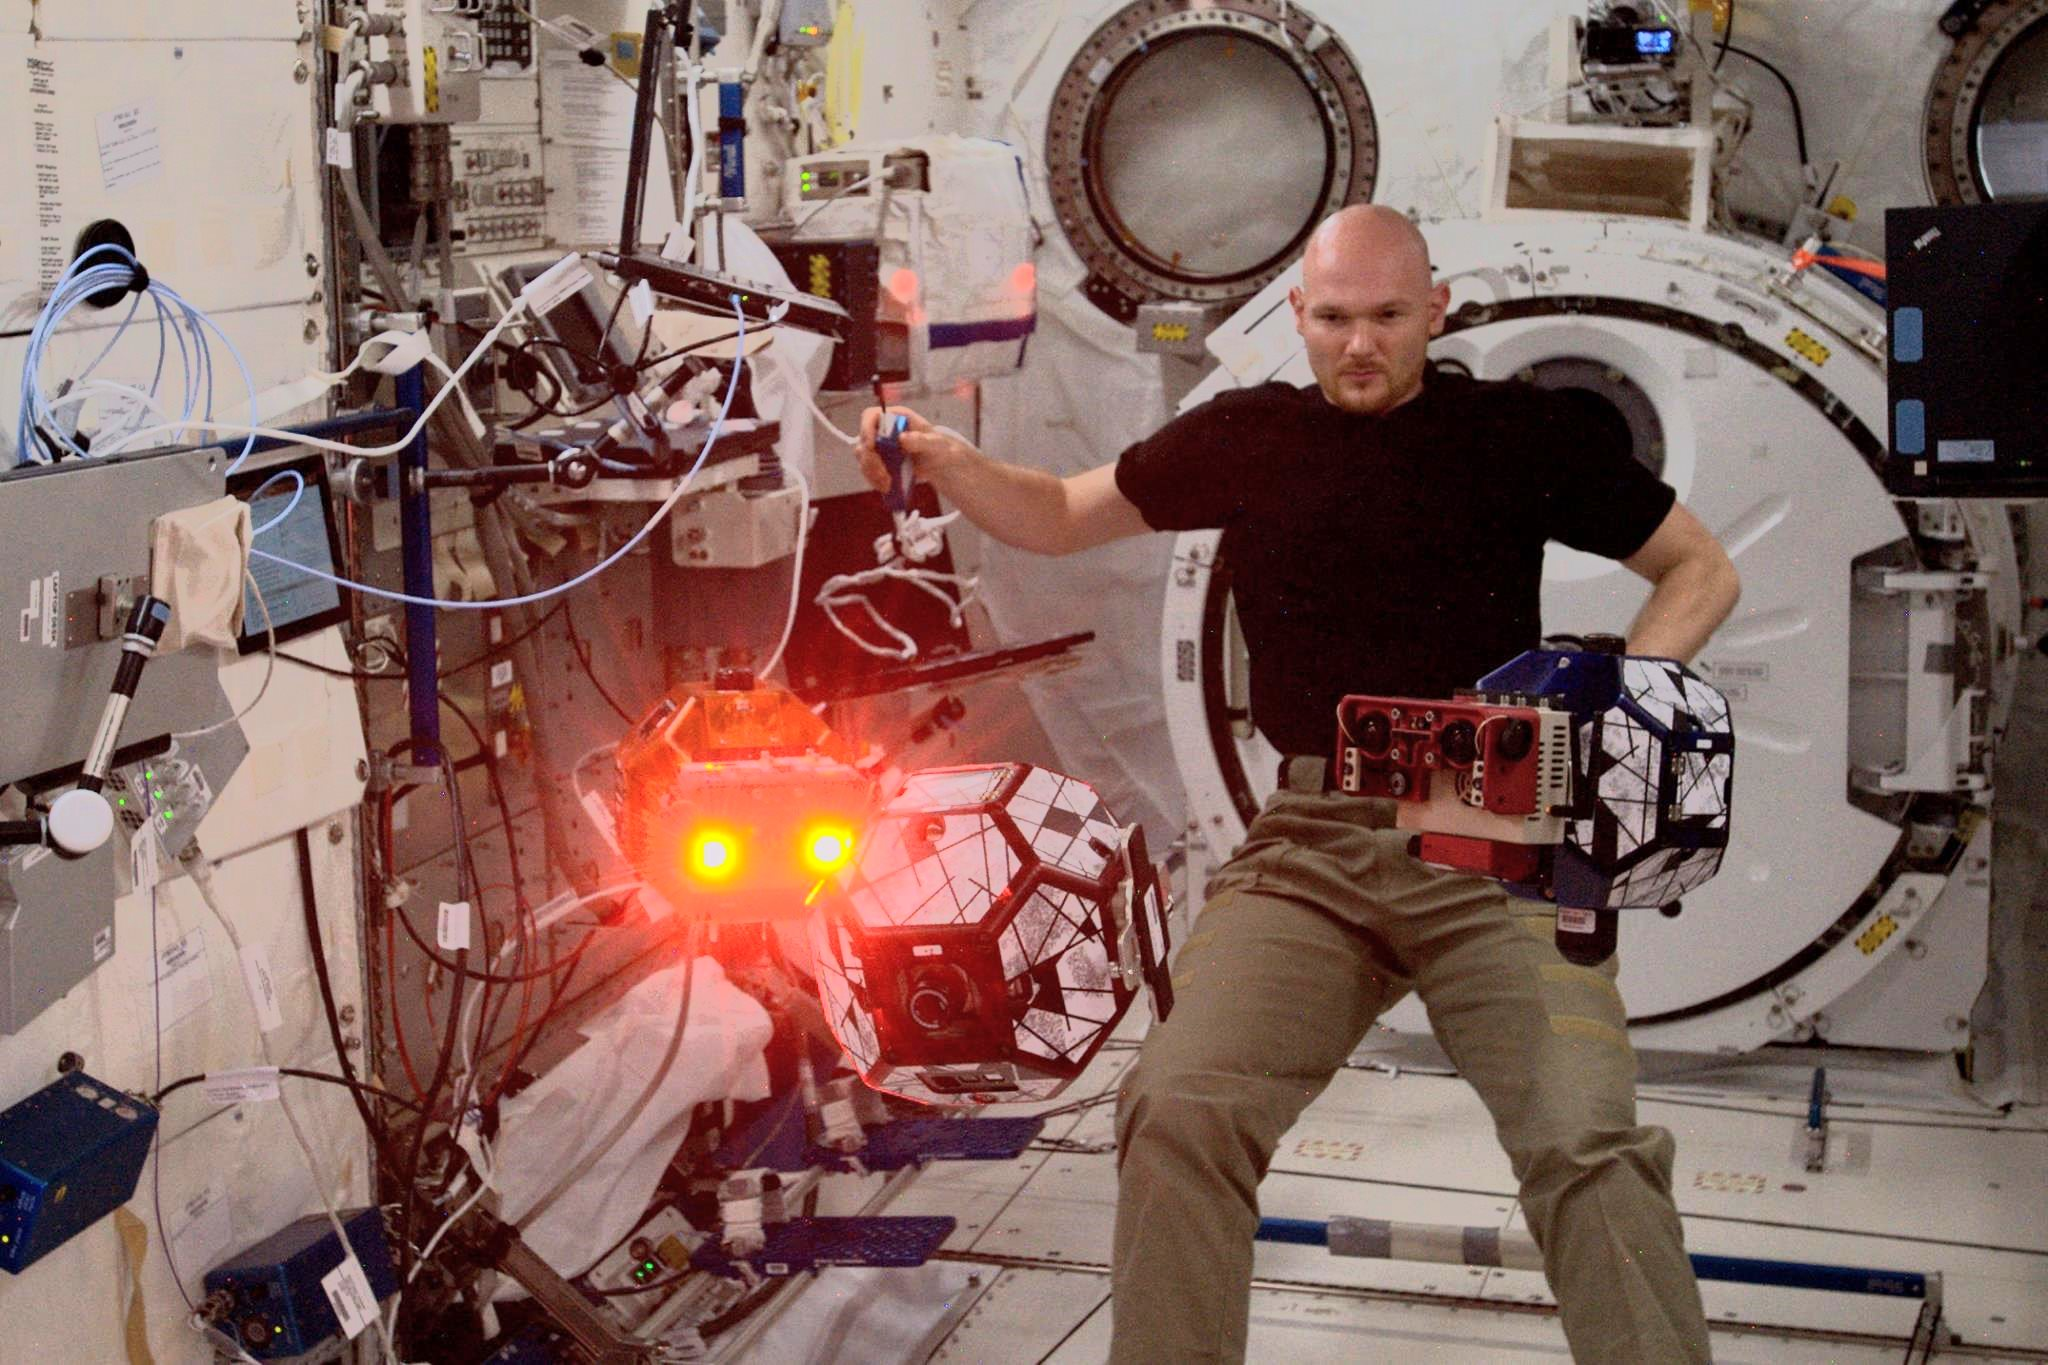
\includegraphics[width=7.5cm]{img/vertigo2.jpg}
\end{subfigure}
\caption{\textit{Left}: the \gls{VERTIGO} stack and goggles with a few explanations. \textit{Right}; a test session in the \gls{ISS} with two \gls{SPHERES} equipped with the \gls{VERTIGO} hardware.}
\label{fig:vertigo}
\end{center}
\end{figure}

\subsection{Halo}
Halo is a ring-shaped structure that is fastened around a \gls{SPHERES} satellite and electrically connected to the \gls{VERTIGO} computer. The structure is made out of several pieces of 3D-printed plastic and provides 22W of electrical power, 2 USB ports and one 1 Gb/s data connection to each one of the 6 expansion ports on the outer face of the ring. Using standardized interface and connector, a wide variety of robotic peripherals can be connected to the satellite, increasing the capability and flexibility of \gls{SPHERES}, and allowing for a wider range of experiments to be conducted. A Time-of-Flight Camera (\gls{ToF}) also called Optical Range Finder (\gls{ORF}), a thermocamera and Control Moment Gyroscopes have been tested as part of the \gls{INSPECT} program to augment the capabilities of an inspector satellite.
\begin{figure}[!htt]
	\begin{center}
		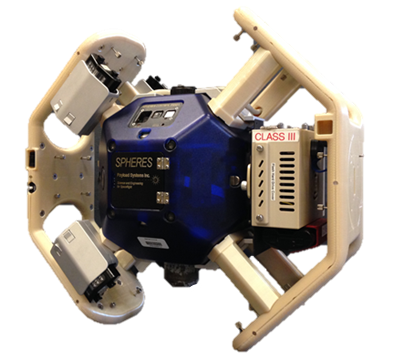
\includegraphics[width=9cm]{img/halo.png}
		\caption{The Halo structure plugged around a \gls{SPHERES} nano-satellite.}
		\label{fig:hal}
	\end{center}
\end{figure}

\newpage

\subsection{\gls{INSPECT}}
The NASA Human Exploration and Operations Mission Directorate (HEOMD) is invested in researching technologies that could reduce risks associated with astronaut spacewalks. One of these is an autonomous system capable of inspecting the exterior of space hardware, a common reason for sending an astronaut outside of the \gls{ISS}. The \gls{INSPECT} system, an Integrated Navigation Sensor Platform for Extravehicular Control and Testing, has been developed as a first step in the progression towards developing a system capable of operating outside of the \gls{ISS} and serving the \gls{HEOMD}'s needs. The sensors on \gls{INSPECT} were selected to fulfill the mission-level requirements to reduce risk by testing capability inside of the \gls{ISS} prior to moving into the vacuum of space.
\begin{figure}[!htt]
\begin{center}
\begin{subfigure}{7cm}
  \centering
  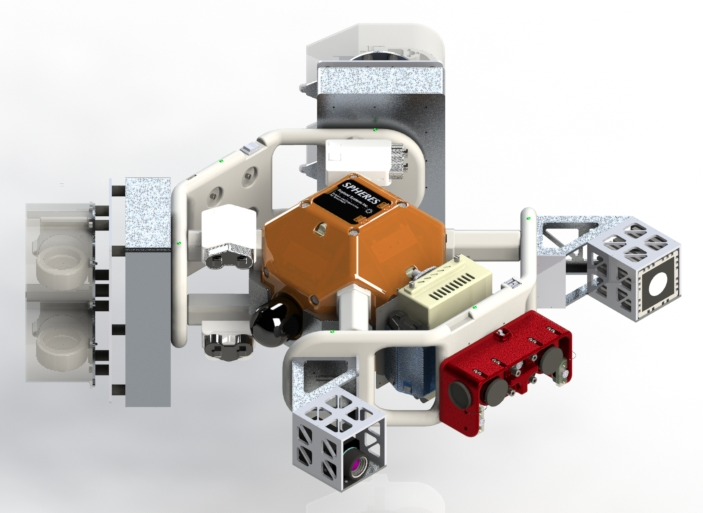
\includegraphics[width=6.9cm]{img/inspect.png}
\end{subfigure}%
\begin{subfigure}{7.5cm}
  \centering
  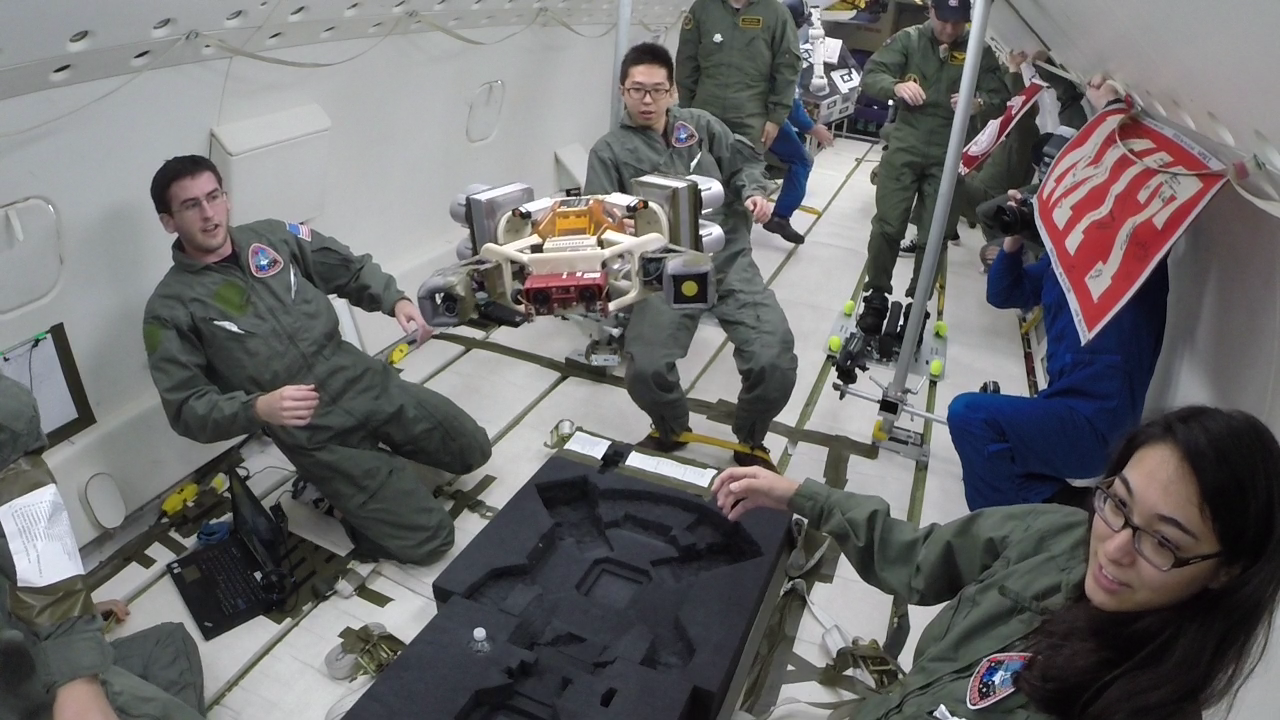
\includegraphics[width=7.4cm]{img/inspect2.png}
\end{subfigure}
\caption{\textit{Left}: a CAD model of the Halo proto-flight equipped with the four cameras and \gls{CMG}'s of the \gls{INSPECT} project. \textit{Right}: a \gls{RGA} parabolic flight test session in July 2014 running the acquisition software developed during this internship.}
\label{fig:inspect}
\end{center}
\end{figure}

\subsection{Testing Environments}
\gls{SPHERES} takes advantage of three different environments to test new control and sensing algorithms as well as new pieces of hardware. In the \textit{ground laboratory}, three \gls{SPHERES} robots can move freely on an air-cushion table around three degrees of freedom (DoF). Besides, \textit{parabolic flights} provided by NASA allow short test sessions in six \gls{DoF}. Finally, in \textit{the \gls{ISS}}, groups of \gls{SPHERES} tests are run by a crew member in test sessions which occur approximately once every three months.

\section{Objectives}
The goal of this work is to create a fusion algorithm taking advantage of \gls{VERTIGO} stereo cameras and the \gls{ORF} camera to provide a 3D cloud with a better accuracy and completeness than the one provided by each sensors separately and to demonstrate the feasibility of this algorithm on the ground and during a Reduced Gravity Aircraft (\gls{RGA}) parabolic flights campaign.

\subsection{Sensors}
\label{subsec:sensors}
The sensors used in this project are part of a selection performed in previous projects in order to answer precise performance and Technology Readiness Levels (\gls{TRL}). Their features are described in table \ref{table:sensors}.
\begin{table}[H]
\begin{center}
\footnotesize
\begin{tabular}{|l|c|c|c|}
\hline
 & \textbf{Stereo cameras} & \textbf{\gls{ORF}} & \textbf{Thermocam}\\
\hline
Brand & IDS-Imaging & MESA-Imaging & FLIR\\
\hline
Model & 2x uEye LE 1225-M-HQ & SwissRange 4000 & A5\\
\hline
Frequency Domain & $717 nm$ dominant (visible) & $850 nm$ (far IR) & $7.5-13 \mu m$ (near IR) \\
\hline
Resolution & 752x480 pixels & 176x144 pixels & 80x64 pixels\\
\hline
Pixel size & $6 \mu m$ & $40 \mu m$& $50 \mu m$\\
\hline
FPS & 10 FPS (typical) to 87 FPS (max) & 10 to 30 FPS (typical) & 60 FPS (typical)\\
\hline
Range & N/A & 0.1m to 7m & N/A\\
\hline
Horizontal \gls{FoV} & 35 degrees & 69 degrees & 44 degrees\\
\hline
Vertical \gls{FoV} & 35 degrees & 55 degrees & 36 degrees\\
\hline
Focal length &  & $10 mm$ (typical) & $5 mm$ (fixed)\\
\hline
Output Data & 10 bits monochrome & 14 bits depth, 16 bits visual & 8 bits monochrome\\
 & &  16 bits confidence & \\
\hline
\end{tabular}
\end{center}
\caption{Brief summary of the sensors characteristics.}\label{table:sensors}
\end{table}

\subsection{Global Architecture}
This fusion algorithm and more broadly the machine vision of the \gls{SPHERES} nano-satellites is part of a \gls{SLAM} algorithm aiming at localizing the robots as well as mapping and understanding the geometry and the motion parameters of objects around the satellite (figure \ref{fig:arch}). Besides, in visual navigation, the outputs of this process are also the inputs of a motion control algorithm which can only be fully tested in zero-gravity environments. Therefore, in this topic, the motion of objects (defined by space dynamics) and the performance associated should be taken into account during the analysis of the results. Moreover, the luminous environment the satellite will evolve in is also very specific, especially during \gls{EVA}, and particular attention on adaptivity to various conditions will be attached during test sessions.

\begin{figure}[!htt]
\begin{center}
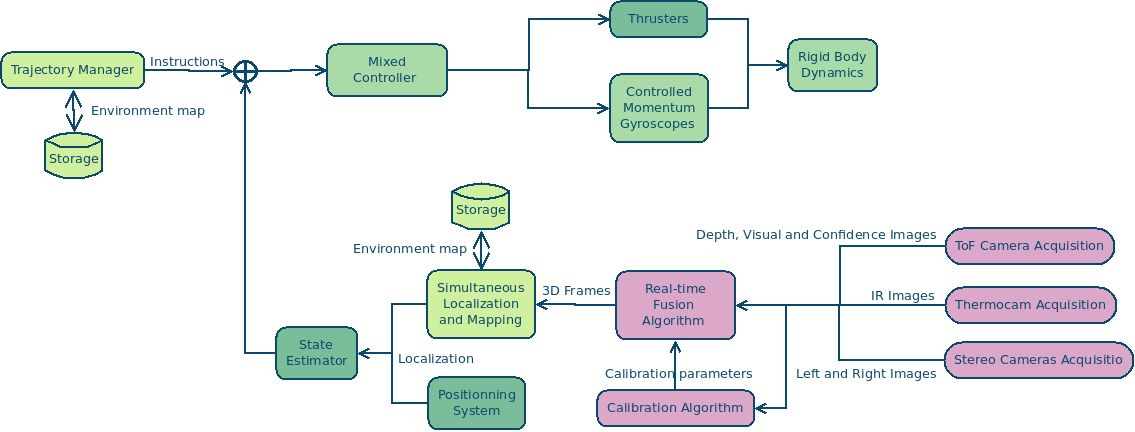
\includegraphics[width=16cm]{img/arch2.png}
\caption{The algorithms developed in this thesis (in rose), situated in the control process of the \gls{INSPECT} project. Sensor fusion 3D frames outputs are directly used in a \gls{SLAM} process which to provide localization estimation but also a useful map for the trajectory manager.}
\label{fig:arch}
\end{center}
\end{figure}


